Dans cette partie nous allons apliquer la méthode de résolution de Newton-Raphson afin de trouver l'équilibre électrostatique d'un système constitué de $N$ charges libres se situant aux positions $x_{1},x_{2},...,x_{N}$ dans l'intervale $[-1,1]$. Notre objectif est donc de déterminer un extremum de la fonction de l'énergie totale du système $E$ qui s'exprime par:
\begin{equation}
  E(x_{1},x_{2},...,x{N}) =  \summation{N}{i=1}(log|x_{i}+1| + log|x_{i} -1 + \frac{1}{2}\summation{N}{j=1,j \neq i} log|x_{i} - x{j}| 
\end{equation}
Cela ce traduit par la résolution de l'équation non-linéaire :
\begin{equation}
  \label{eq:eq1}
  \begin{split}
  \nabla E(x_{1},x_{2},...,x_{N}) = 0
  \end{split}
\end{equation}

\subsection{Calcul de la matrice Jacobienne de $\nabla E$}
Après simplification de l'expression du gradient de la fonction d'énergie totale on obtient : 
\begin{equation}
  \label{eq:gradient}
  \begin{split}
    \nabla E(x_{1},x_{2},...,x_{N})  & = \left( \frac{\partial E }{\partial x_{i}}\right)_{1 \leq i \leq N} \\
    & = \left(\frac{1}{x_{i}+1} + \frac{1}{x_{i} -1} + \frac{1}{2} \summation{N}{j=1,j\neq i}\frac{1}{x_{i}-x{j}}\right)_{1 \leq i \leq N }
  \end{split}
\end{equation}
On note $J$ la matrice Jacobienne de $\nabla E$
on a d'après \ref{eq:gradient} :
\begin{equation}
  \label{eq:jacobian}
  \begin{split}
    J & = \left(\frac{\partial \nabla E }{\partial x_{i} \partial x_{j}}\right)_{1 \leq i \leq N , 1 \leq j \leq N} \\
    & = \left\{
    \begin{array}{ll}
      -\frac{1}{(x_{i}+1)^{2}} - \frac{1}{(x_{i} -1)^{2}} - \frac{1}{2} \summation{N}{j=1,j\neq i}\frac{1}{(x_{i}-x{j})^{2}}& \mbox{si i = j} \\
      -\frac{1}{2(x_{i} - x{j})^{2}} & \mbox{sinon} 
    \end{array}
    \right.
  \end{split}  
\end{equation}

En Python, les deux fonctions sont mises en œuvre et l'algorithme de Newton-Raphson est appliqué en utilisant la fonction $\nabla E(x_1, x_2, \cdots , x_N)$ et la fonction qui calcule sa Jacobienne définie par l'équation \eqref{eq:jacobian}. Le résultat est un vecteur dont les coordonnées sont les solutions de l'équation \eqref{eq:eq1}. La figure \ref{fig:legendre} illustre ces solutions placées sur l'axe des réels, avec en surimpression les dérivées des polynômes de Legendre d'ordre 1 à 6. On peut constater que les racines des dérivées correspondent approximativement aux coordonnées du vecteur solution.

\begin{figure}[H]
  \centering
  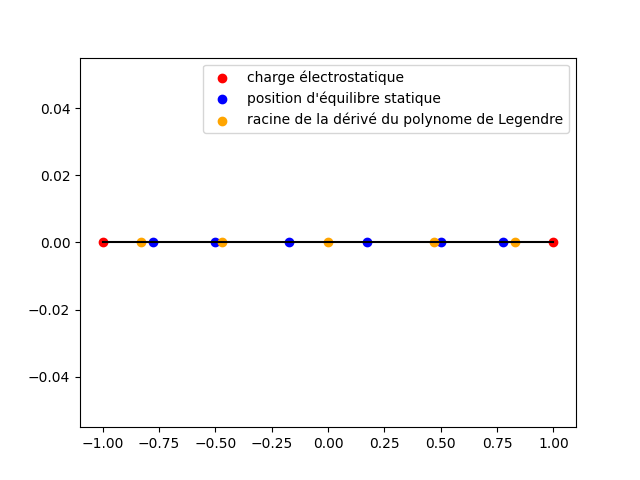
\includegraphics[width=0.5\textwidth]{img/legendre.png}
  \caption{Vecteur solution positionné sur l'axe des réels, superposé avec les racines de la dérivées des polynomes de Legendre d'ordre 1 à 6}
  \label{fig:legendre}
\end{figure}

Pour évaluer si la solution correspond à un maximum ou à un minimum, on s'est appuyé sur les valeurs propres de la matrice jacobienne $J_{\nabla E}$, calculée pour le vecteur contenant les positions d'équilibre. Étant donné que toutes les valeurs propres sont négatives, on peut conclure que la solution correspond à un maximum.


